\section{Kinematics for the Da vinci robot}

% \begin{figure}
% 		\centering
% 		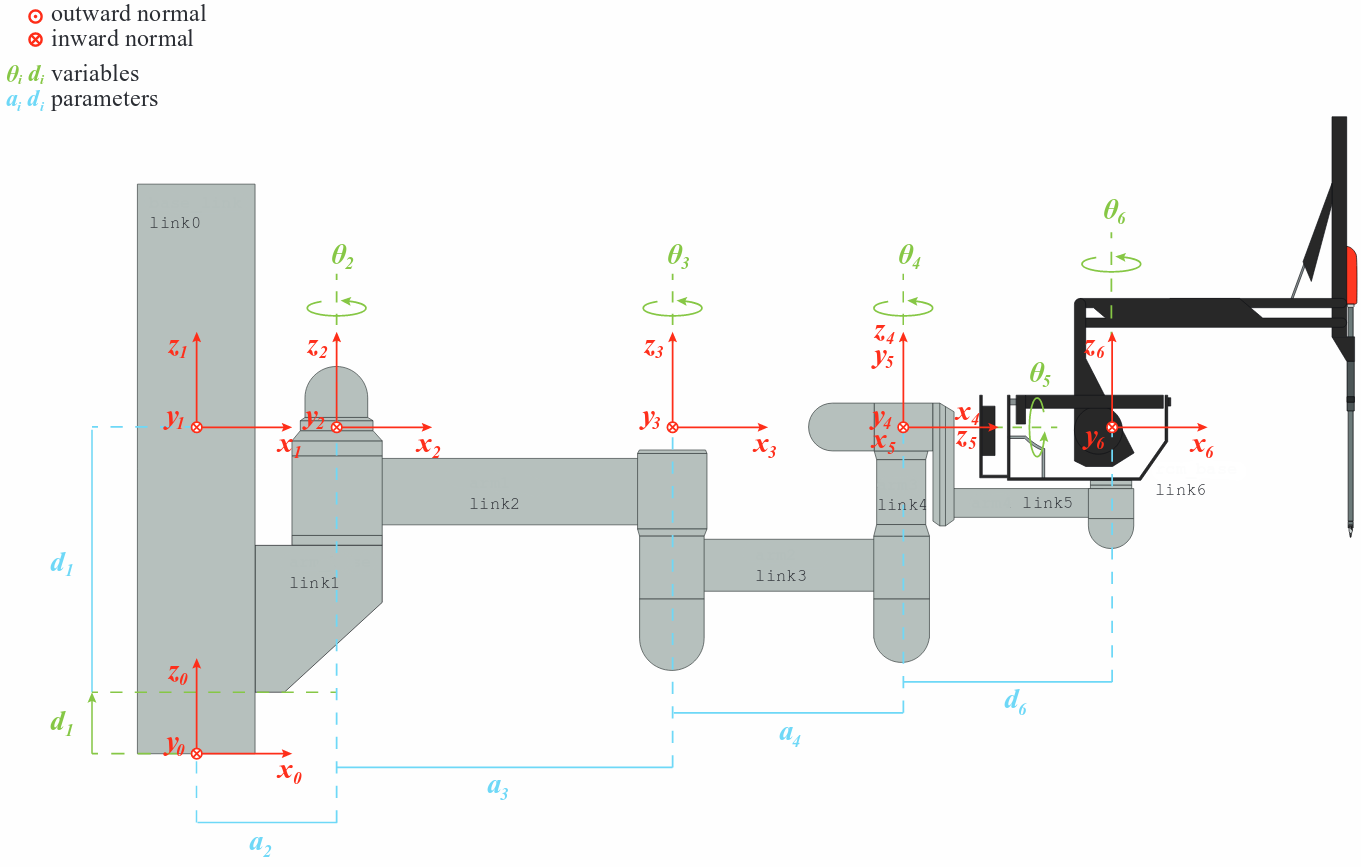
\includegraphics[width=1.2\linewidth]{da_arm.png}
% 		\caption{Show different joints and their attached frame coordinate}
% 		\label{fig:da_ha_en}
% \end{figure}

% \begin{figure}
% 		\centering
% 		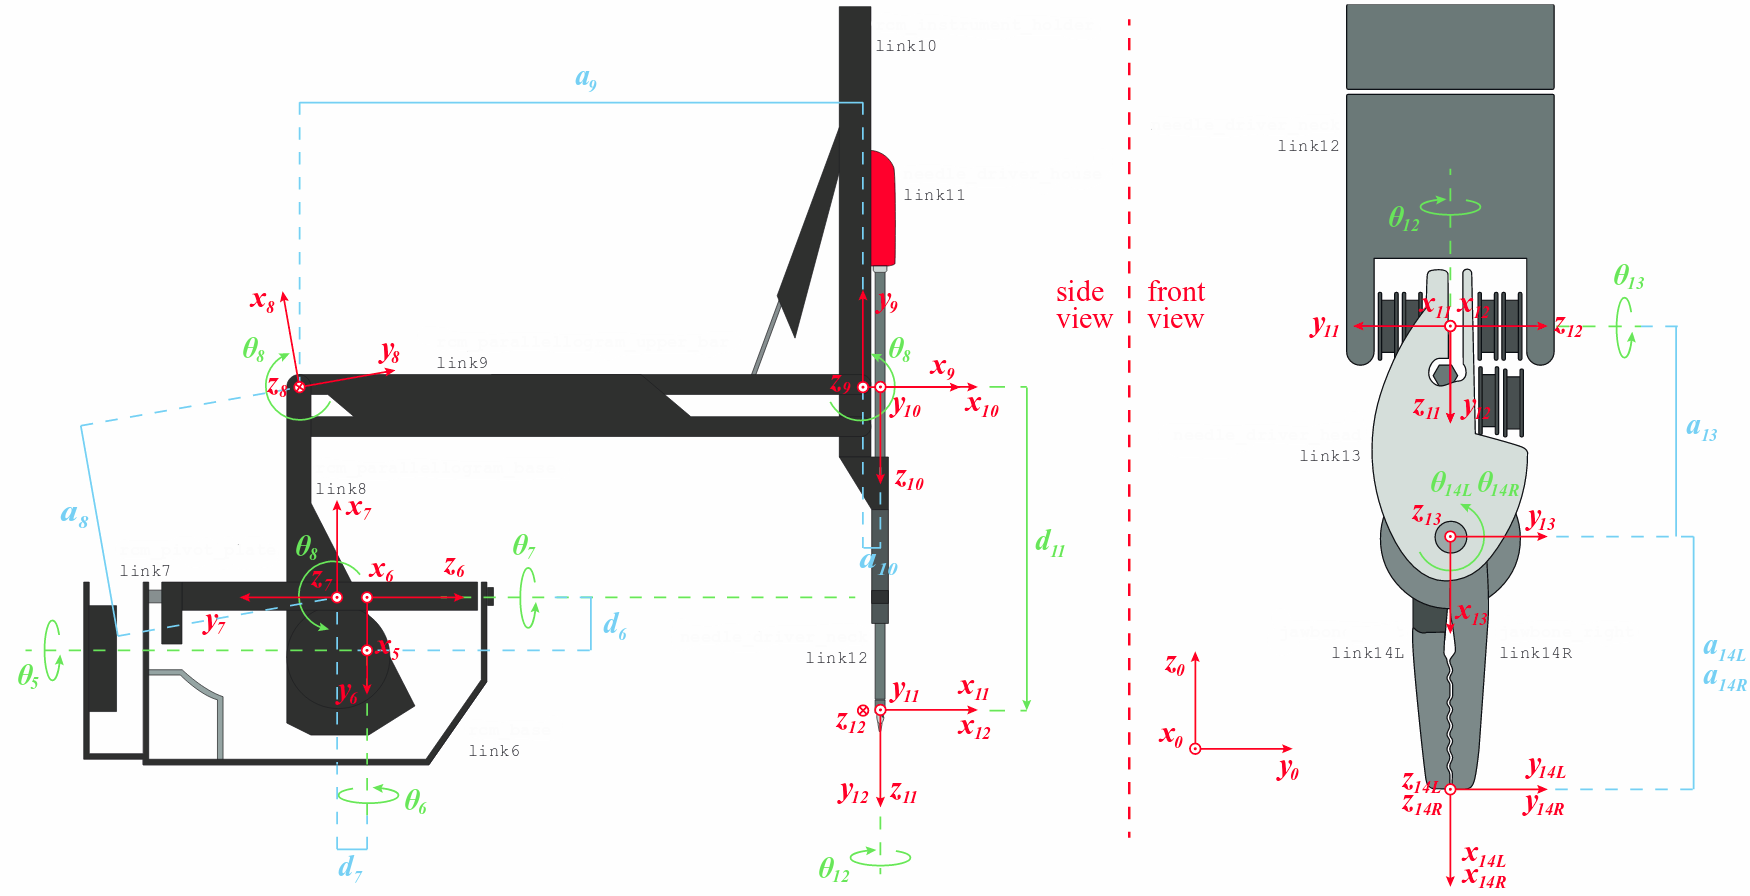
\includegraphics[width=1.2\linewidth]{Davinci_hand_endo.png}
% 		\caption{Show different joints and their attached frame coordinate}
% 		\label{fig:da_ha_en}
% \end{figure}

\begin{sidewaysfigure}
		\centering
		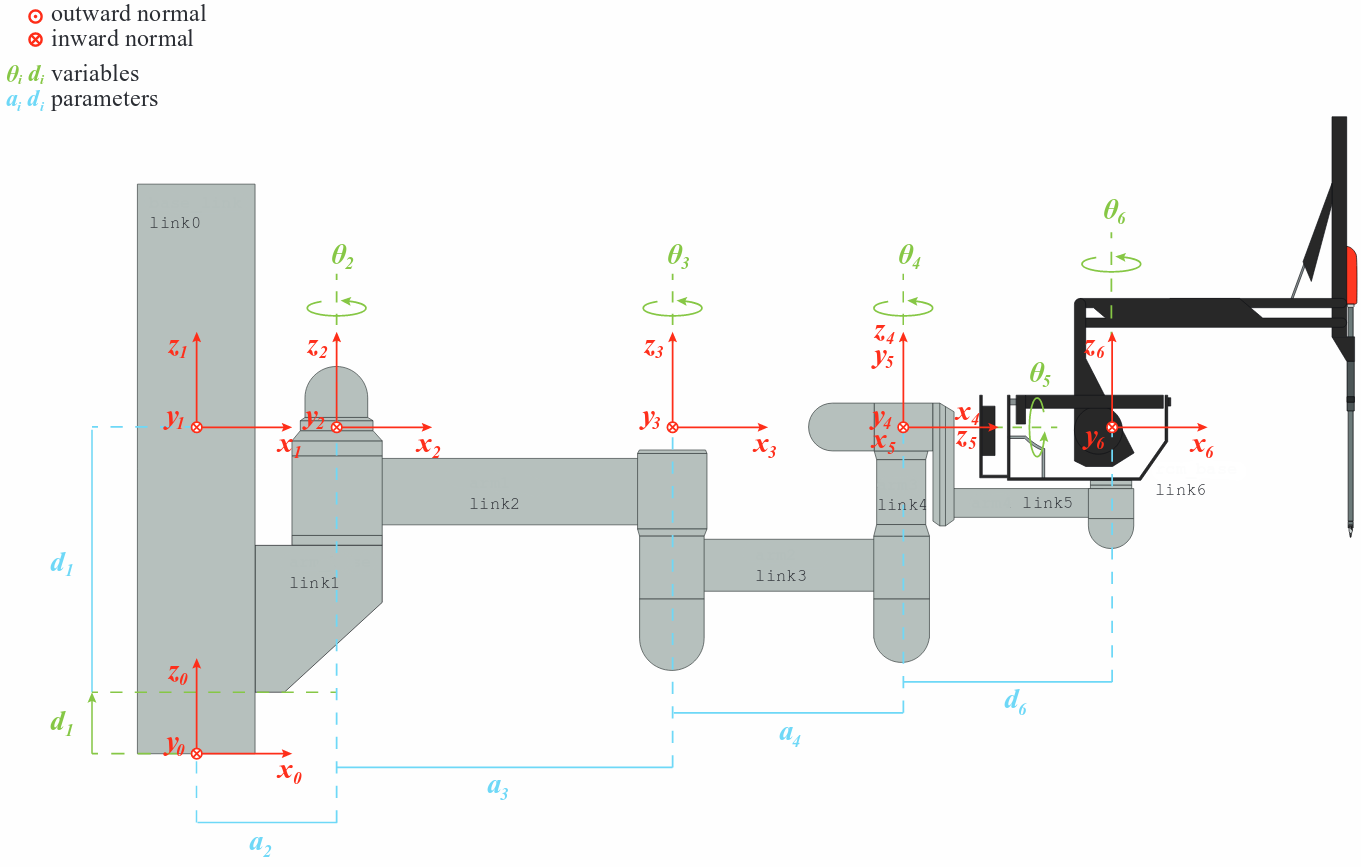
\includegraphics[width=0.9\linewidth]{da_arm.png}
		\caption{Show different joints and their attached frame coordinate}
		\label{fig:da_ha_en}
\end{sidewaysfigure}


%stolen from page 108:
%projekter.aau.dk/projekter/files/213514652/Safety_in_Automated_Surgery_with_the_da_Vinci_Robot.pdf

\todo{Better resulution}
\todoc{Do we have to draw this our self or is it okay just to make a ref to stolen location}
\begin{sidewaysfigure}
		\centering
		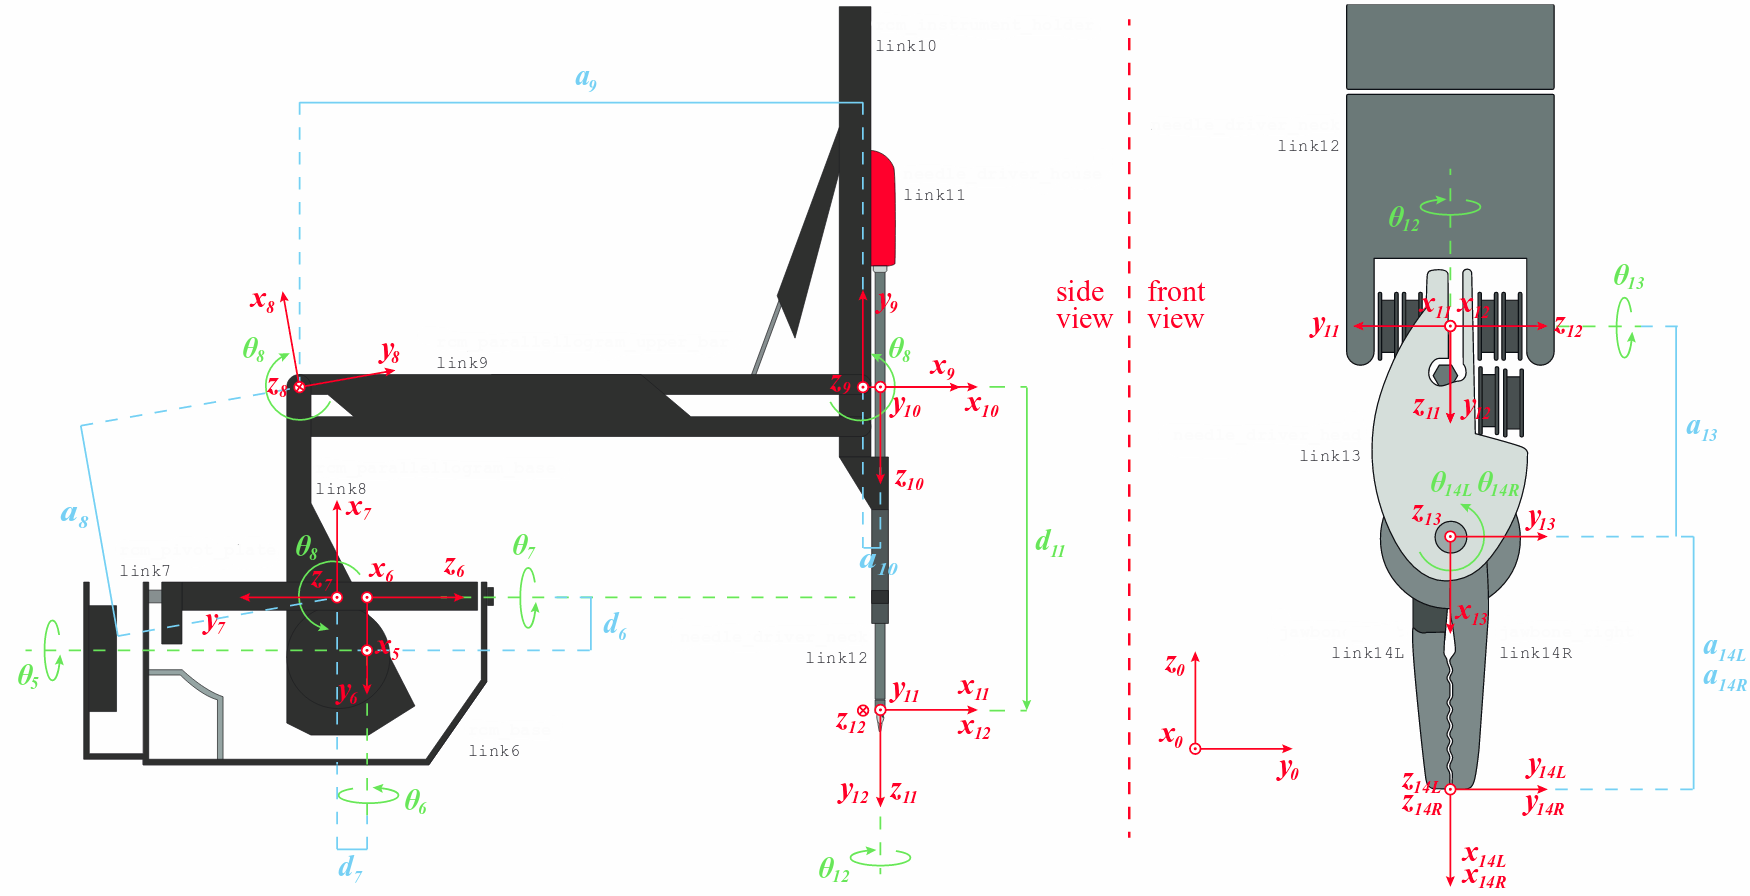
\includegraphics[width=1\linewidth]{Davinci_hand_endo.png}
		\caption{Show different joints and their attached frame coordinate}
		\label{fig:da_ha_en}
\end{sidewaysfigure}

